\documentclass{article}

\usepackage{fancyhdr}
\usepackage{extramarks}
\usepackage{amsmath}
\usepackage{amsthm}
\usepackage{amsfonts}
\usepackage{tikz}
\usepackage[plain]{algorithm}
\usepackage{algpseudocode}
\usepackage{enumerate}
\usepackage{amssymb}

\usetikzlibrary{automata,positioning}

%
% Basic Document Settings
%

\topmargin=-0.45in
\evensidemargin=0in
\oddsidemargin=0in
\textwidth=6.5in
\textheight=9.0in
\headsep=0.25in

\linespread{1.1}

\pagestyle{fancy}
\lhead{\hmwkAuthorName}
\chead{\hmwkClass\ (\hmwkClassInstructor\ \hmwkClassTime): \hmwkTitle}
\rhead{\firstxmark}
\lfoot{\lastxmark}
\cfoot{\thepage}

\renewcommand\headrulewidth{0.4pt}
\renewcommand\footrulewidth{0.4pt}

\setlength\parindent{0pt}

%
% Create Problem Sections
%

\newcommand{\enterProblemHeader}[1]{
    \nobreak\extramarks{}{Problem \arabic{#1} continued on next page\ldots}\nobreak{}
    \nobreak\extramarks{Problem \arabic{#1} (continued)}{Problem \arabic{#1} continued on next page\ldots}\nobreak{}
}

\newcommand{\exitProblemHeader}[1]{
    \nobreak\extramarks{Problem \arabic{#1} (continued)}{Problem \arabic{#1} continued on next page\ldots}\nobreak{}
    \stepcounter{#1}
    \nobreak\extramarks{Problem \arabic{#1}}{}\nobreak{}
}

\setcounter{secnumdepth}{0}
\newcounter{partCounter}
\newcounter{homeworkProblemCounter}
\setcounter{homeworkProblemCounter}{1}
\nobreak\extramarks{Problem \arabic{homeworkProblemCounter}}{}\nobreak{}

%
% Homework Problem Environment
%
% This environment takes an optional argument. When given, it will adjust the
% problem counter. This is useful for when the problems given for your
% assignment aren't sequential. See the last 3 problems of this template for an
% example.
%
\newenvironment{homeworkProblem}[1][-1]{
    \ifnum#1>0
        \setcounter{homeworkProblemCounter}{#1}
    \fi
    \section{Problem \arabic{homeworkProblemCounter}}
    \setcounter{partCounter}{1}
    \enterProblemHeader{homeworkProblemCounter}
}{
    \exitProblemHeader{homeworkProblemCounter}
}

%
% Homework Details
%   - Title
%   - Due date
%   - Class
%   - Section/Time
%   - Instructor
%   - Author
%

\newcommand{\hmwkTitle}{Tutorial 11}
\newcommand{\hmwkDueDate}{April 6, 2021}
\newcommand{\hmwkClass}{CZ2003}
\newcommand{\hmwkClassTime}{SS3}
\newcommand{\hmwkClassInstructor}{Assoc Prof Alexei Sourin}
\newcommand{\hmwkAuthorName}{\textbf{Pang Yu Shao}}
\newcommand{\hmwkAuthorID}{\textbf{U1721680D}}

%
% Title Page
%

\title{
    \vspace{2in}
    \textmd{\textbf{\hmwkClass:\ \hmwkTitle}}\\
    \normalsize\vspace{0.1in}\small{Due\ on\ \hmwkDueDate\ at 10:30am}\\
    \vspace{0.1in}\large{\textit{\hmwkClassInstructor\ - \hmwkClassTime}}
    \vspace{3in}\\
    \hmwkAuthorName\\
    \hmwkAuthorID
}

\date{05/04/2021}

\renewcommand{\part}[1]{\textbf{\large Part \Alph{partCounter}}\stepcounter{partCounter}\\}

%
% Various Helper Commands
%

% Useful for algorithms
\newcommand{\alg}[1]{\textsc{\bfseries \footnotesize #1}}

% For derivatives
\newcommand{\deriv}[1]{\frac{\mathrm{d}}{\mathrm{d}x} (#1)}

% For partial derivatives
\newcommand{\pderiv}[2]{\frac{\partial}{\partial #1} (#2)}

% Integral dx
\newcommand{\dx}{\mathrm{d}x}

% Alias for the Solution section header
\newcommand{\solution}{\textbf{\large Solution}}

% Probability commands: Expectation, Variance, Covariance, Bias
\newcommand{\E}{\mathrm{E}}
\newcommand{\Var}{\mathrm{Var}}
\newcommand{\Cov}{\mathrm{Cov}}
\newcommand{\Bias}{\mathrm{Bias}}

\begin{document}

\maketitle

\pagebreak

\begin{homeworkProblem}
   Which three components does the Phong illumination model contain? Which of them 
   will change if one of the followings happens in a scene?\\
   \begin{enumerate}[a]
      \item A light source is moved to a new location.
      \item The object is moved to a new location.
      \item The observer is moved to a new location.
   \end{enumerate}
   \textbf{Solution}\\
   The Phong illumination model contains the 3 components: \textbf{Ambient reflection},
   \textbf{Diffuse reflection} and \textbf{Specular reflection}.
   \begin{displaymath}
      I = K_aI_a + k_dI_s(N \cdot L) + k_sI_s(V \cdot R)^n
   \end{displaymath}

   If the light source is moved to a new location, Diffuse and Specular reflection would be changed.\\\\

   If the object is moved to a new location, Diffuse and Specular reflection would be changed.\\\\

   If the observer is moved to a new location, only the Specular reflection would be changed.\\\\




\end{homeworkProblem}
\pagebreak
\begin{homeworkProblem}
   What is the value of the specular exponent for a perfect mirror? Why?\\\\
   \textbf{Solution}\\
   In a perfect mirror, the concentration of the specular highlight would be high 
   and the highlight would have a sharp drop off,

   In this case, the specular exponent would be infinitely high $n = \infty$

    
\end{homeworkProblem}

\pagebreak
\begin{homeworkProblem}
   A plane is defined by the equation $x + z - 2 = 0$, with the diffuse reflection
   coefficient 0.5. A point light source with intensity 1 is located at $(10, 10, 10)$.
   Calculate a diffuse reflection on the plane at point $(1,10,1)$.\\\\
   \textbf{Solution}\\
   The diffuse reflection component of Phong illumination model can be obtained using 
   the following $k_dI_s(N\cdot L)$, where $k_d = 0.5$, $I_s = 1$ \\\\

   $N = \frac{(A, B, C)}{\sqrt{A^2 + B^2 + C^2}}$\\
   $N = \frac{(1, 0, 1)}{\sqrt{2}} = (\frac{\sqrt{2}}{2}, 0, \frac{\sqrt{2}}{2}) $\\\\

   Lighting vector: $L = (10, 10, 10) - (1, 10, 1) = (9,  0, 9)$\\
   After Normalisation, $L = \frac{(9, 0, 9)}{\sqrt{9^2 + 9^2}} = (\frac{\sqrt{2}}{2}, 0, \frac{\sqrt{2}}{2})$\\\\

   Therefore, \\
   $k_dI_s(N\cdot L) = (0.5*1)(\frac{\sqrt{2}}{2}*\frac{\sqrt{2}}{2} + \frac{\sqrt{2}}{2}*\frac{\sqrt{2}}{2})$\\
   $= 0.5* (0.5 + 0.5)$\\
   $= \mathbf{0.5}$







   

\end{homeworkProblem}

\pagebreak
\begin{homeworkProblem}
   A point light source with intensity 1 is located at coordinates $(8, 10, 10)$. It
illuminates an origin-centered sphere with radius 2, diffuse coefficient 0.7, specular
coefficient 0.2, and specular exponent 2. The ambient reflection coefficient is 0.1.
The intensity of the ambient light source is 1. An observer located at the position
with coordinates $(10, 0, 0)$ is looking at a point on the sphere, along the direction $[-
1\ 0\ 0]$. Find the point and calculate the illumination on the surface of the sphere at
the point seen by the observer.
   \begin{figure}[H]
      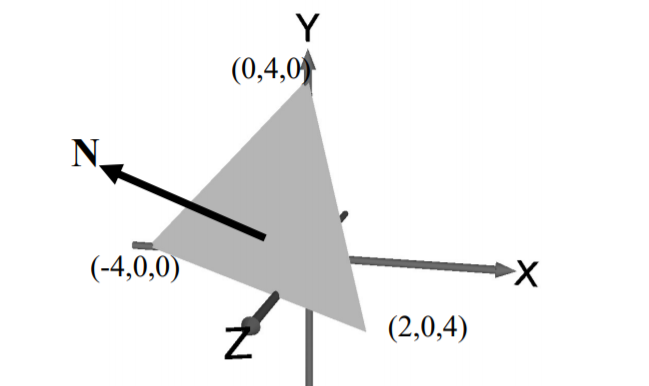
\includegraphics[width=8cm]{fig/q4.PNG}
      \centering
   \end{figure}
   \textbf{Solution}\\

   $I = K_aI_a + k_dI_s(N \cdot L) + k_sI_s(V \cdot R)^n$\\
   $k_a = 0.1$, $I_a = 1$, $k_d = 0.7$, $I_s = 1$, $k_s = 0.2$, $n = 2$\\\\

   Observer is looking at point (2, 0, 0) on the sphere.\\
   $\vec{N} = \frac{(2, 0, 0)}{2} = (1, 0, 0)$\\\\

   Calculating light vector L:\\
   $\vec{L} = (8,10,10) - (2,0,0) = (6, 10, 10)$\\
   After normalisation:\\
   $\vec{L} = \frac{(6, 10, 10)}{\sqrt{236}} = (0.3906, 0.6509, 0.6509)$\\\\

   Calculating viewing vector V:\\
   $\vec{V} = (10,0,0) - (2,0,0) = (8, 0, 0)$\\
   After normalisation:\\
   $\vec{V} = (1,0,0)$\\\\

   Calculating reflected vector R:\\
   $\vec{R} = 2(N\cdot L)N - L$\\
   $\vec{R} = 2(0.3906)N - L$\\
   $\vec{R} = 0.7811(1,0,0) - (0.3906, 0.6509, 0.6509) = (0.3906, -0.6509, -0.6509)$\\\\
   
   Therefore,\\
   $\vec{N}\cdot\vec{L} = (1, 0, 0)\cdot(0.3906, 0.6509, 0.6509) = 0.3906$\\
   $\vec{V}\cdot\vec{R} = (1, 0, 0)\cdot(0.3906, -0.6509, -0.6509) = 0.3906$\\\\

   $I = 0.1 + 0.7(0.3906) + 0.2(0.3906)^2$\\
   $= \mathbf{0.4039}$
\end{homeworkProblem}

\end{document}